\documentclass[11pt,a4paper]{article}

\usepackage[T1]{fontenc}
\usepackage[utf8]{inputenc}
\usepackage[brazilian]{babel}
\usepackage{amsmath,amssymb}
\usepackage{booktabs}
\usepackage{graphicx}
\usepackage{placeins}
\usepackage{listings}
\usepackage{geometry}
\usepackage[hidelinks]{hyperref}
\geometry{margin=2.5cm}

\title{\textbf{Atividade 3 -- RBFNet com Duplicatas e Regularização}\\[1.2em]\large Aprendizado Computacional e Reconhecimento de Padrões}
\author{Caique Frederico Pereira de Moura}
\date{23 de abril de 2026}

\lstset{
	language=Python,
	basicstyle=\ttfamily\small,
	breaklines=true,
	frame=single
}

\begin{document}

\maketitle
\tableofcontents
\newpage

\section{Objetivo da atividade}

Este relatório apresenta a implementação e a análise de duas abordagens: (i) RBFNet com regularização para lidar com duplicatas na base de treino e (ii) pipeline \textbf{PolyMap-RBFNet-SVMLin}, com comparação sistemática entre bases e métodos.

\section{Tópico 1 -- RBFNet com duplicatas}

\subsection{Problema numérico}

No treinamento supervisionado da RBFNet com erro quadrático (SSE), os pesos da camada de saída podem ser obtidos pela solução fechada:

\begin{equation}
\mathbf{w} = (\Phi^T\Phi)^{-1}\Phi^T\mathbf{y},
\end{equation}

em que $\Phi$ é a matriz de ativações da camada RBF. Quando há padrões idênticos na base, colunas/linhas de $\Phi$ podem ficar linearmente dependentes, tornando $\Phi^T\Phi$ singular ou mal condicionada.

\subsection{Estratégia proposta}

A estratégia adotada foi a \textbf{regularização de Tikhonov (Ridge)} na etapa supervisionada:

\begin{equation}
\mathbf{w} = (\Phi^T\Phi + \lambda I)^{-1}\Phi^T\mathbf{y}, \quad \lambda > 0.
\end{equation}

Essa modificação desloca os autovalores da matriz normal e reduz o número de condição, aumentando a estabilidade numérica sem alterar a estrutura da RBFNet.

\subsection{Implementação}

Foi usado o conjunto artificial solicitado:

\begin{lstlisting}
X, y = make_moons(n_samples=500, noise=0.1, random_state=42)
X = np.vstack([X, X[:20]])
y = np.hstack([y, y[:20]])
\end{lstlisting}

No notebook, a classe RBFNet foi implementada com centros por KMeans e estimação regularizada dos pesos:

\begin{lstlisting}
I = np.eye(Phi.shape[1])
self.weights = np.linalg.inv(Phi.T @ Phi + self.lambd * I) @ Phi.T @ y
\end{lstlisting}

Configuração principal do experimento: $n\_centers = 15$, $\sigma = 0.5$, divisão treino/teste 70/30 e $\lambda = 10^{-2}$ para o modelo final.

\section{Tópico 2 -- PolyMap-RBFNet-SVMLin}

Nesta etapa, foi implementado o processo combinado \textbf{PolyMap-RBFNet-SVMLin}, seguindo exatamente as quatro fases solicitadas.

\subsection{Etapas do método}

\begin{enumerate}
\item Remapeamento polinomial: os dados originais em $\mathbb{R}^n$ são transformados para $\mathbb{R}^q$ via \texttt{PolynomialFeatures(degree=d)}.
\item Camada RBF (fase não supervisionada): com os dados remapeados, define-se o número de centros como
\begin{equation}
N_c = d \cdot q,
\end{equation}
e os centros são obtidos por KMeans.
\item Classificação linear: as ativações RBF alimentam um SVM linear com penalidade $C$ e estratégia OVR.
\item Avaliação: o desempenho final é medido pelo percentual de acerto (acurácia).
\end{enumerate}

\subsection{Resumo da implementação}

No notebook, o fluxo foi implementado por uma função no formato:

\begin{lstlisting}
def poly_rbf_svm(X, y, d=2, C=1.0, sigma=1.0):
	X_train, X_test, y_train, y_test = train_test_split(
		X, y, test_size=0.3, random_state=42
	)

	poly = PolynomialFeatures(degree=d)
	X_train_poly = poly.fit_transform(X_train)
	X_test_poly = poly.transform(X_test)

	q = X_train_poly.shape[1]
	n_centers = d * q

	centers = KMeans(n_clusters=n_centers, random_state=42).fit(
		X_train_poly
	).cluster_centers_

	Phi_train = rbf(X_train_poly, centers, sigma)
	Phi_test = rbf(X_test_poly, centers, sigma)

	svm = LinearSVC(C=C, max_iter=10000)
	svm.fit(Phi_train, y_train)

	y_pred = svm.predict(Phi_test)
	return accuracy_score(y_test, y_pred)
\end{lstlisting}

\subsection{Resultados gráficos}

\begin{figure}[htbp]
\centering
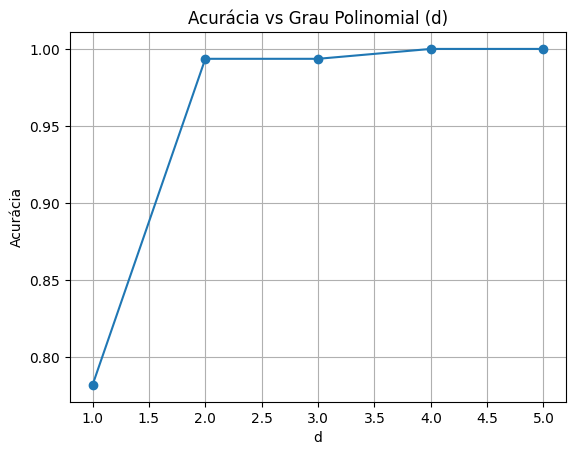
\includegraphics[width=1.0625\textwidth,height=7.5cm,keepaspectratio]{plot_acuracia_vs_d.png}
\caption{Acurácia em função do grau polinomial $d$.}
\label{fig:acc-vs-d}
\end{figure}

\begin{figure}[htbp]
\centering
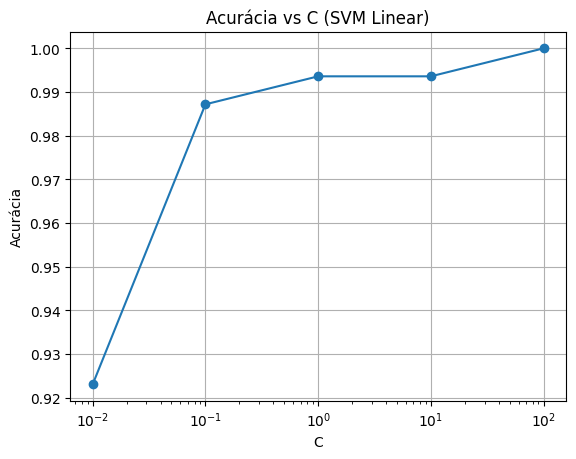
\includegraphics[width=1.0625\textwidth,height=7.5cm,keepaspectratio]{plot_acuracia_vs_C.png}
\caption{Acurácia em função de $C$ no SVM linear.}
\label{fig:acc-vs-c}
\end{figure}

\begin{figure}[htbp]
\centering
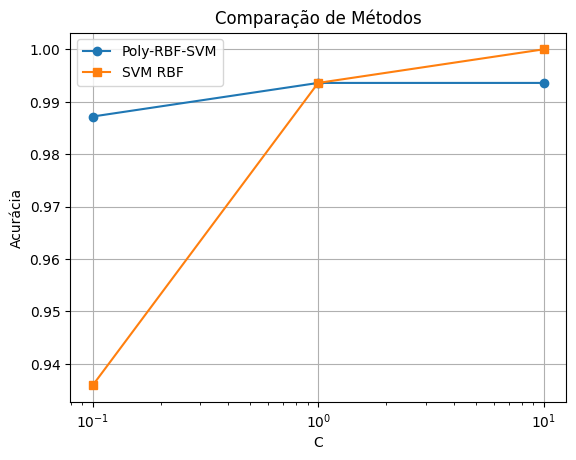
\includegraphics[width=1.0625\textwidth,height=7.5cm,keepaspectratio]{plot_comparacao_metodos.png}
\caption{Comparação entre PolyMap-RBFNet-SVMLin e SVM-RBF.}
\label{fig:comparacao-metodos}
\end{figure}

\FloatBarrier

\section{Tópico 3 -- Aplicação em Wine, Iris e base do Exercício 1}

\subsection{Objetivo}

Aplicar o método \textbf{PolyMap-RBFNet-SVMLin} às bases \textit{Wine Dataset}, \textit{Iris Dataset} e à base sintética do Tópico 1, analisando o efeito dos parâmetros $d$ e $C$. Em paralelo, comparar os percentuais de acerto com o método SVM com kernel RBF para diferentes valores de $C$ e $\gamma$.

\subsection{Heatmaps SVM-RBF}

\begin{figure}[htbp]
\centering
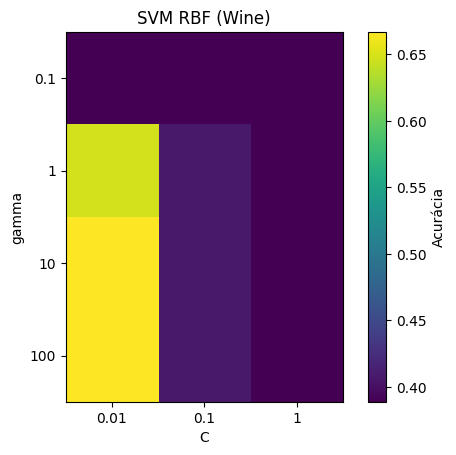
\includegraphics[width=1.0625\textwidth,height=7.5cm,keepaspectratio]{heatmap_rbf_wine.png}
\caption{Heatmap de acurácia do RBF-SVM na base Wine - Não normalizado.}
\label{fig:t3-wine}
\end{figure}

\begin{figure}[htbp]
\centering
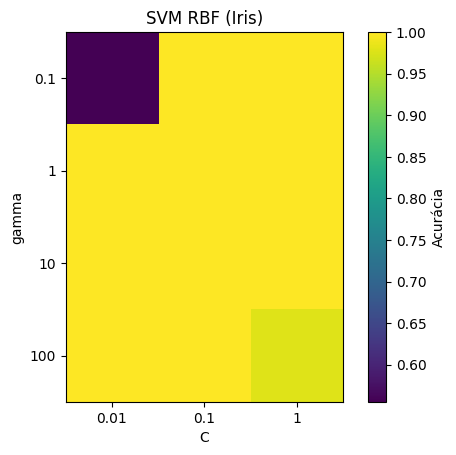
\includegraphics[width=1.0625\textwidth,height=7.5cm,keepaspectratio]{heatmap_svm_iris.png}
\caption{Heatmap de acurácia do RBF-SVM na base Iris.}
\label{fig:t3-iris}
\end{figure}

\begin{figure}[htbp]
\centering
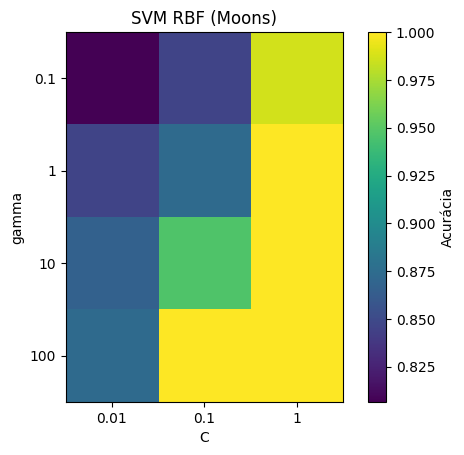
\includegraphics[width=1.0625\textwidth,height=7.5cm,keepaspectratio]{heatmap_svm_moons.png}
\caption{Heatmap de acurácia do RBF-SVM na base sintética (Moons).}
\label{fig:t3-sintetica}
\end{figure}

\FloatBarrier

\subsection{Heatmaps Poly-RBF-SVM}

\begin{figure}[htbp]
\centering
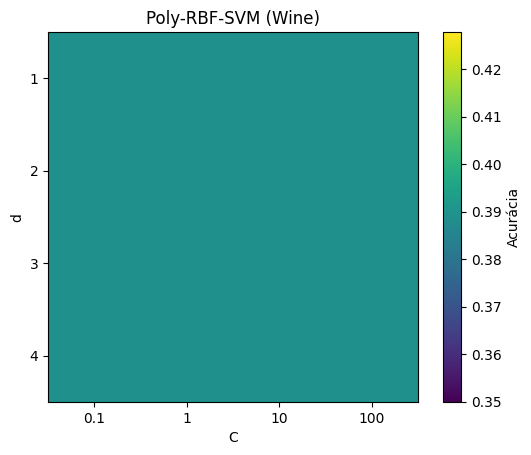
\includegraphics[width=1.0625\textwidth,height=7.5cm,keepaspectratio]{heatmap_wine.png}
\caption{Heatmap de acurácia do Poly-RBF-SVM na base Wine - Não normalizado.}
\label{fig:t3-heatmap-wine}
\end{figure}

\begin{figure}[htbp]
\centering
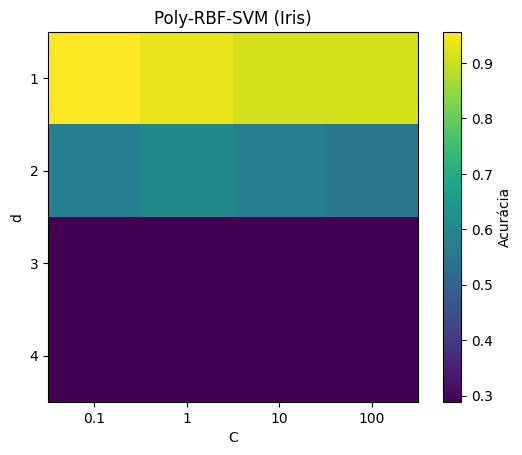
\includegraphics[width=1.0625\textwidth,height=7.5cm,keepaspectratio]{heatmap_iris.png}
\caption{Heatmap de acurácia do Poly-RBF-SVM na base Iris.}
\label{fig:t3-heatmap-iris}
\end{figure}

\begin{figure}[htbp]
\centering
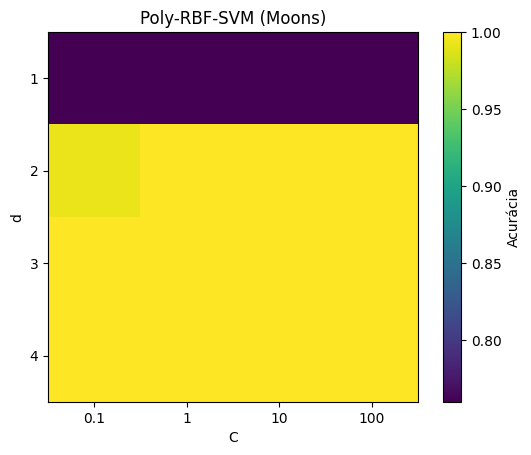
\includegraphics[width=1.0625\textwidth,height=7.5cm,keepaspectratio]{heatmap_moons.png}
\caption{Heatmap de acurácia do Poly-RBF-SVM na base sintética (Moons).}
\label{fig:t3-heatmap-moons}
\end{figure}

\FloatBarrier

\section{Resultados e discussão}

Considerando o \textbf{Tópico 1}, a regularização Ridge mostrou-se efetiva para estabilizar o treinamento supervisionado da RBFNet na presença de amostras repetidas. Mesmo com padrões idênticos na base, a modelagem permaneceu numericamente estável, com redução da sensibilidade dos pesos e manutenção de alto desempenho preditivo.

No \textbf{Tópico 2}, os gráficos de variação de $d$ e $C$ indicam que a abordagem PolyMap-RBFNet-SVMLin é sensível à escolha de hiperparâmetros, mas apresenta comportamento consistente em faixas intermediárias. A análise visual por curvas e heatmap reforça que a combinação entre remapeamento polinomial e camada RBF pode ampliar a capacidade discriminativa quando os parâmetros são bem ajustados.

No \textbf{Tópico 3}, a comparação entre bases (Wine, Iris e sintética) mostra que o método proposto mantém desempenho competitivo frente ao SVM com kernel RBF. Em termos práticos, o SVM-RBF tende a apresentar maior robustez global, enquanto o PolyMap-RBFNet-SVMLin oferece maior flexibilidade na construção explícita do espaço de características, o que pode ser vantajoso para análise e controle do modelo, porém com maior custo de ajuste.

De forma integrada, os resultados sugerem um compromisso entre \textbf{estabilidade e simplicidade} (SVM-RBF) e \textbf{flexibilidade de representação} (PolyMap-RBFNet-SVMLin), com desempenho final dependente do cenário e da calibração de $d$, $C$ e $\gamma$.

\section{Conclusão}

Observa-se que o método PolyMap-RBFNet-SVMLin apresenta desempenho competitivo em relação ao SVM com kernel RBF, especialmente para valores intermediários de $d$ e $C$. No entanto, o SVM RBF tende a ser mais estável, uma vez que seu kernel já incorpora implicitamente transformações não lineares. Por outro lado, a abordagem proposta permite maior controle sobre a construção do espaço de características, ao custo de maior complexidade e sensibilidade à escolha dos parâmetros.

\end{document}
